%-*- TeX -*- -*- Soft -*-,
% http://www.gigasciencejournal.com/authors/instructions/commentary 

\documentclass[11pt]{bmc_article_s50}

\usepackage{amsthm,amsmath}
\usepackage{siunitx}
\usepackage[colorinlistoftodos]{todonotes}
\usepackage[utf8]{inputenc}
\RequirePackage{hyperref}
\usepackage{array}
\newcolumntype{L}[1]{>{\raggedright\let\newline\\\arraybackslash\hspace{0pt}}p{#1}}
\newcolumntype{R}[1]{>{\raggedleft\let\newline\\\arraybackslash\hspace{0pt}}p{#1}}
\usepackage{longtable}
\usepackage{booktabs}
\usepackage{url}
\urlstyle{rm}
\usepackage{setspace}
\usepackage[T1]{fontenc}
\pagestyle{empty}
\setlength{\parindent}{0cm}
\usepackage{ragged2e}
\justifying
\singlespace

\parskip = 0pt
\captionsetup{labelfont=bf,labelsep=period,singlelinecheck=off}

\begin{document} % (800-1200 words)

\title{Brainhack: a collaborative workshop for the open neuroscience community}
\maketitle

\author[0,1,2*]{R Cameron Craddock}\cor{}\email{ccraddock@nki.rfmh.org}
\author[0,3]{Daniel S Margulies}\email{margulies@cbs.mpg.de}
\author[0,5,13]{Pierre Bellec}\email{pierre.bellec@criugm.qc.ca}
\textbf{\textcolor{red}{[AU: Authors' affiliations should be listed in strict ascending numerical order. Please check and change.]}}

\author[0,6,7]{B Nolan Nichols}\email{nolan.nichols@gmail.com}
\author[8]{Sarael Alcauter}\email{alcauter@gmail.com}
\author[8]{Fernando A Barrios}\email{fbarrios@unam.mx}
\author[9,10]{Yves Burnod}\email{yburnod@gmail.com}
\author[11]{Christopher J Cannistraci}\email{Christopher.Cannistraci@mssm.edu}
\author[12,13]{Julien Cohen-Adad}\email{jcohen@polymtl.ca}
\author[12]{Benjamin De Leener}\email{benjamin.de-leener@polymtl.ca}
\author[14]{Sebastien Dery}\email{sderymail@gmail.com}
\author[15,16,17]{Jonathan Downar}\email{Jonathan.Downar@uhn.ca}
\author[15,17]{Katharine Dunlop}\email{katharine.dunlop@gmail.com}
\author[0,18,19,20]{Alexandre R Franco}\email{alexandre.franco@pucrs.br}
\author[0,1]{Caroline Seligman Froehlich}\email{cfroehlich@nki.rfmh.org}
\author[21,22]{Andrew J Gerber}\email{GerberA@nyspi.columbia.edu}
\author[0,23,51]{Satrajit S Ghosh}\email{satra@mit.edu}
\author[24,25]{Thomas J Grabowski}\email{tgrabow@uw.edu}
\author[26,27]{Sean Hill}\email{sean.hill@incf.org}
\author[34]{Anibal S\'{o}lon Heinsfeld}\email{anibal.heinsfeld@acad.pucrs.br}
\author[0,28]{R Matthew Hutchison}\email{rhutchison@fas.harvard.edu}
\author[0,11]{Prantik Kundu}\email{prantik.kundu@mssm.edu}
\author[31]{Angela R Laird}\email{alaird@fiu.edu}
\author[0,29,30]{Sook-Lei Liew}\email{sliew@usc.edu}
\author[32]{Daniel J Lurie}\email{danjlurie@gmail.com}
\author[0,33,52]{Donald G McLaren}\email{donald@biospective.com}
\author[34]{Felipe Meneguzzi}\email{felipe.meneguzzi@pucrs.br}
\author[0,35]{Maarten Mennes}\email{mennes.maarten@gmail.com}
\author[10,36]{Salma Mesmoudi}\email{salma.mesmoudi@gmail.com}
\author[2]{David O'Connor}\email{david.oconnor@childmind.org}
\author[8]{Erick H Pasaye}\email{pasayeric@hotmail.com}
\author[37]{Scott Peltier}\email{spelt@umich.edu}
\author[38,39]{Jean-Baptiste Poline}\email{jbpoline@gmail.com}
\author[40]{Gautam Prasad}\email{gautam.prasad@loni.usc.edu}
\author[34]{Ramon Fraga Pereira}\email{ramon.pereira@acad.pucrs.br}
\author[4]{Pierre-Olivier Quirion}\email{pioliqui@gmail.com}
\author[41]{Ariel Rokem}\email{arokem@gmail.com}
\author[42]{Ziad S Saad}\email{ziad.ss@gmail.com}
\author[40]{Yonggang Shi}\email{yonggang.shi@loni.usc.edu}
\author[43,44,45]{Stephen C Strother}\email{sstrother@research.baycrest.org}
\author[0,46,47]{Roberto Toro}\email{rto@pasteur.fr}
\author[0,48,49]{Lucina Q Uddin}\email{l.uddin@miami.edu}
\author[30]{John D Van Horn}\email{jvanhorn@usc.edu}
\author[50]{John W Van Meter}\email{john.vanmeter.phd@gmail.com}
\author[53,54]{Robert C Welsh}\email{rcwelsh@umich.edu}
\author[2]{Ting Xu}\email{ting.xu@childmind.org}

\address[0]{
  The Neuro Bureau\\
\textbf{\textcolor{red}{\hspace*{59pt}[AU: Start addresses at 1 rather than 0?\\\hspace*{59pt}Is there an address to go with this affiliation?]}}
}
\address[1]{
  Computational Neuroimaging Lab, Center for Biomedical Imaging and\\\hspace*{59pt} Neuromodulation, Nathan S. Kline Institute for Psychiatric Research,\\\hspace*{59pt} Orangeburg, New York, USA\\
\textbf{\textcolor{red}{\hspace*{59pt}[AU: Please supply zip codes for all addresses.]}}
}
\address[2]{
  Center for the Developing Brain, Child Mind Institute, New York, New York, USA
}
\address[3]{
  Max Planck Research Group for Neuroanatomy \& Connectivity, Max Planck Institute\\\hspace*{59pt} for Human Cognitive and Brain Sciences, Leipzig, Germany
}
\address[4]{
  \textbf{\textcolor{red}{[AU: Please supply the details for address 4.]}}
}
\address[5]{
  D\'epartement d'Informatique et de Recherche Op\'erationnelle, Universit\'e de Montr\'eal,\\\hspace*{59pt} Montr\'eal, Qu\'{e}bec, Canada
}
\address[6]{
  Center for Health Sciences, SRI International, Menlo Park,  California, USA
}
\address[7]{
  Department of Psychiatry and Behavioral Sciences, Stanford University,\\\hspace*{59pt} Stanford,  California, USA
}
\address[8]{
  Instituto De Neurobiolog\'{i}a, Universidad Nacional Aut\'{o}noma de M\'{e}xico,\\\hspace*{59pt} Quer\'{e}taro, M\'{e}xico
}
\address[9]{
  Laboratoire d'Imagerie Biomédicale, Sorbonne Universités, UPMC\\\hspace*{59pt} Université Paris 06, Paris, France
}
\address[10]{
  Institut des Systèmes Complexes de Paris-Île-de-France, Paris, France
}
\address[11]{
  Translational and Molecular Imaging Institute, Icahn School of Medicine at Mount Sinai,\\\hspace*{59pt} New York, New York, USA
}
\address[12]{
  Institute of Biomedical Engineering, Ecole Polytechnique de Montr\'{e}al, Montr\'{e}al,\\\hspace*{59pt} Qu\'{e}bec, Canada
}
\address[13]{
  Functional Neuroimaging Unit, Centre de Recherche de l'Institut Universitaire de\\\hspace*{59pt} G\'eriatrie de Montr\'eal, Montr\'{e}al, Qu\'{e}bec, Canada
}
\address[14]{
  McConnell Brain Imaging Center, Montreal Neurological Institute, McGill University,\\\hspace*{59pt} Montreal, Quebec, Canada
}
\address[15]{
   MRI-Guided rTMS Clinic, University Health Network, Toronto, Ontario, Canada
}
\address[16]{
  Department of Psychiatry, University Health Network, University of Toronto,\\\hspace*{59pt} Toronto, Ontario, Canada
}
\address[17]{
  Institute of Medical Sciences, University of Toronto, Toronto, Ontario, Canada
}
\address[18]{
  Faculdade de Engenharia,  PUCRS, Porto Alegre, Brazil
}
\address[19]{
  Instituto do C\'{e}rebro do Rio Grande do Sul, PUCRS, Porto Alegre, Brazil
}
\address[20]{
  Faculdade de Medicina, PUCRS, Brazil
}
\address[21]{
  New York State Psychiatric Institute, New York, New York, USA
}
\address[22]{
  Division of Child and Adolescent Psychiatry, Department of Psychiatry,\\\hspace*{59pt} Columbia University, New York, New York, USA
}
\address[23]{
  McGovern Institute for Brain Research, Massachusetts Institute of Technology,\\\hspace*{59pt} Cambridge, Massachusetts, USA
}
\address[24]{
  Department of Radiology, University of Washington, Seattle, Washington, USA
}
\address[25]{
  Department of Neurology, University of Washington, Seattle, Washington, USA
}
\address[26]{
  International Neuroinformatics Coordinating Facility, Stockholm, Sweden
}
\address[27]{
  Karolinska Institutet, Stockholm, Sweden
}
\address[28]{
  Center for Brain Science, Harvard University, Cambridge, Massachusetts, USA
}
\address[29]{
  Chan Division of Occupational Science and Occupational Therapy, Division of\\\hspace*{59pt} Physical Therapy and Biokinesiology, Department of Neurology, University of\\\hspace*{59pt} Southern California, Los Angeles, California, USA
}
\address[30]{
  USC Mark and Mary Stevens Neuroimaging and Informatics Institute, University\\\hspace*{59pt} of Southern California, Los Angeles, Canada, USA
}
\address[31]{
  Department of Physics, Florida International University, Miami, Florida, USA
}
\address[32]{
  Department of Psychology, University of California, Berkeley, California, USA
}
\address[33]{
  Biospective, Inc., Montr\'{e}al, Qu\'{e}bec, Canada
}
\address[34]{
  Faculdade de Inform\'{a}tica, PUCRS, Porto Alegre, Brazil
}
\address[35]{
  Radboud University Nijmegen, Donders Institute for Brain, Cognition and Behaviour,\\\hspace*{59pt} Centre for Cognitive Neuroimaging, Nijmegen, The Netherlands.
}
\address[36]{
  Sorbonne Universit\'{e}s, Paris-1 Universit\'{e}, Equipement d'Excellence MATRICE,\\\hspace*{59pt} Paris, France
}
\address[37]{
  Functional MRI Laboratory, University of Michigan, Ann Arbor, Michigan, USA
}
\address[38]{
  Helen Wills Neuroscience Institute, University of California, Berkeley,\\\hspace*{59pt} California, USA
}
\address[39]{
  Henry H. Wheeler Jr. Brain Imaging Center, University of California, Berkeley,\\\hspace*{59pt} California, USA
}
\address[40]{
  Laboratory of Neuro Imaging, Stevens Neuroimaging and Informatics Institute,\\\hspace*{59pt} Keck School of Medicine  of University of Southern California,\\\hspace*{59pt} Los Angeles, California, USA
}
\address[41]{
  The University of Washington eScience Institute, Seattle, Washington, USA
}
\address[42]{
  Scientific and Statistical Computing Core, National Institute of Mental\\\hspace*{59pt} Health, Bethesda, Maryland, USA %MD
}
\address[43]{
  Rotman Research Institute, Baycrest Hospital, Toronto, Ontario, Canada
}
\address[44]{
  Department of Medical Biophysics, University of Toronto, Toronto, Ontario, Canada
}
\address[45]{
  Institute of Medical Science, University of Toronto, Toronto, Ontario, Canada
}
\address[46]{
   Human Genetics and Cognitive Functions Unit, Institut Pasteur, Paris, France
}
\address[47]{
  Unité Mixte de Recherche 3571, Genes, Synapses and Cognition, Centre\\\hspace*{59pt} National de la Recherche Scientifique, Institut Pasteur, Paris, France
}
\address[48]{
  Department of Psychology, University of Miami, Coral Gables, Florida, USA
}
\address[49]{
 Neuroscience Program, University of Miami Miller School of Medicine,\\\hspace*{59pt} Miami, Florida, USA
}
\address[50]{
  Center for Functional and Molecular Imaging, Georgetown University Medical\\\hspace*{59pt} Center, Washington, DC, USA
}
\address[51]{
  Department of Otology and Laryngology, Harvard Medical School, Boston,\\\hspace*{59pt} Massachusetts, % MA,
 USA
}
\address[52]{
  Department of Neurology, Massachusetts General Hospital, Boston, %MA,
\\\hspace*{59pt}Massachusetts, USA
}
\address[53]{
  Department of Psychiatry, University of Michigan, Ann Arbor, %MI
Michigan, USA
}
\address[54]{
  Department of Radiology, University of Michigan, Ann Arbor, %MI
Michigan, USA
}

\begin{abstract} % (max 100 words)
Brainhack events offer a novel workshop format with participant-generated content that caters to the rapidly growing open neuroscience community. Including components from hackathons and unconferences, as well as parallel educational sessions, Brainhack fosters novel collaborations around the interests of its attendees. Here we provide an overview of its structure, past events, and example projects. Additionally, we outline current innovations such as regional events and post-conference publications. Through introducing Brainhack to the wider neuroscience community, we hope to provide a unique conference format that promotes the features of collaborative, open science.

\end{abstract}

\keywords{hackathon, unconference, open science, neuroscience, data sharing, collaboration, networking}

\parindent = 20pt
\section*{Introducing Brainhack}

Open science promotes collaboration through the transparent dissemination of ideas, tools, and data, with the goal of accelerating the pace of discovery. Although scientific conferences and workshops seem like a natural medium for brain researchers to meet and exchange ideas, in practice these events, often structured around the lecturer--audience paradigm, do not always provide sufficient flexibility or free time to fully exploit their potential. Borne from the technology sector, `unconferences' and `hackathons' are alternative meeting formats that emphasize the full participation of all attendees. Rather than having a prearranged program, the content presented at unconferences is dynamically determined by attendees, 
while hackathons feature unstructured time during which teams of participants collaborate intensively on various projects. These meeting formats have enabled rapid advances in computing technologies since the late 1990s, but they have yet to be widely adopted in academic research. 


Now in their fourth year, international and regional Brainhack events bring together brain enthusiasts from a variety of backgrounds to build relationships, learn from one another, and collaborate on projects related to the neurosciences. Unlike traditional hackathons that tend to focus on computer programming, projects at Brainhacks can be completed using a much broader array of methods. Time is set aside for periodic unconference sessions whose content is determined on-site by the participants. The unconference sessions can feature different styles of presentations, including but not limited to: updates on ongoing projects, ideas that could seed future collaborations, panel discussions, or tutorials. In consideration of the ever expanding interest in the tools of open science, Brainhack has developed an educational component that runs in parallel %to
with the hacking sessions in order to introduce the basic tools of open collaboration. This combined model encourages active participation and interaction between attendees, while also maximizing the topical relevance of the more formally presented content (see Figure~\ref{fig1}).

\begin{figure}[htp]
\begin{center}
  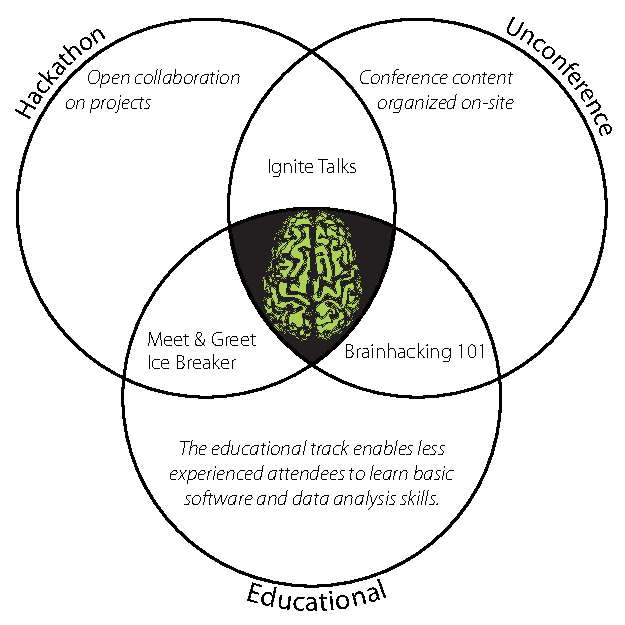
\includegraphics[width=0.5\textwidth]{Figure_01}
  \caption{\href{http://www.brainhack.org}{Brainhack} {\textbf{\textcolor{red}{[AU: Please convert all links to references, cited in the usual way.]}}} is composed of various organizational features from `unconferences' and `hackathons,' and includes a variety of scheduling components to encourage collaboration and introduction to open science methods.}
  \label{fig1}
\end{center}
\end{figure}

% DM: CONSIDER integrating into second paragraph of of section{Brainhack projects}
There is no ideal background, skill set, or experience level required for Brainhack attendees. Fully translating neuroscience data to knowledge requires expertise that spans %across
 biology, computer science, engineering, informatics, mathematics, neuroanatomy, philosophy, physics, psychiatry, psychology, statistics, art, and many others. The goal of a Brainhack event is to facilitate the cross-pollination of ideas and knowledge across these various disciplines and communities to accelerate the development of a richer understanding of the brain. In addition to sharing data and tools, attendees can contribute in a variety of ways. Philosophical debates about the meanings of cognition, coordinated efforts to manually segment brain images from different species, curating neuroscience literature, or helping others to understand the subtleties of diagnosing a developmental disorder are all examples of valuable contributions that have emerged at Brainhacks in the past (for further examples, see Table~\ref{tab3}).

\subsection*{Hackathons based on collaboration, not competition}

The hackathon format gained prominence in the technology sector by providing a meeting model that targets specific project goals during intense time-limited collaborations. The competitive aspect of the traditional hackathon, while catalyzing rapid advances toward specific technology ends, is contrary to the founding %principal
principle of Brainhack, which is to encourage open, cross-institutional, and inter-disciplinary collaboration. Rather than subdividing attendees into competitive factions, Brainhack attendees are encouraged to work together in collaborative teams to solve problems of their choosing. In this way, rather than obtaining many solutions to a single problem, we aim to produce various solutions to many problems. Most importantly, we encourage the building of new relationships that continue to be productive beyond the end of the event.

\subsection*{Brainhack projects}

Rather than focusing on a specific problem or toolset, which is common in traditional hackathons, attendees are encouraged to generate their own project ideas around which they can self-assemble into teams. As a consequence, some projects may receive more limited interest, whereas %another
one might attract the majority of attendees. In this way, the projects developed at Brainhacks are elected by participation, rather than being pre-specified by the event organizers. This model is more conducive to collaboration than the alternative of organizing a hackathon around a challenge or competition. There are many different models between these two extremes; %,
  we are currently working on building thematic Brainhack events that bring researchers together to focus on specific questions of neuroscientific interest.

To date, projects completed at Brainhack events have %spanned from
included students interacting with more experienced researchers to learn about a new data modality or analysis method, inter-disciplinary collaborations to improve data collection, the development or optimization of data analysis tools, %to
and testing hypotheses about brain structure using openly shared data. See Table~\ref{tab3} for selected examples of projects that have previously been initiated at Brainhack events, and \href{http://www.brainhack.org}{www.brainhack.org} {\textbf{\textcolor{red}{[AU: See previous comment re links.]}}} for a full list of projects.

\subsection*{Event organization}

Brainhack events span %one
1 to %four
4~days and include %d
 a variety of content to make them both accessible and fruitful for a wide range of attendees. The format of the events is not fixed, but varies based on the needs determined by the local organizing committee. At past events, the schedule has included various components aiming to quickly integrate the attendees and generate an environment conducive to productive collaboration. We have found the activity categories included in Table~\ref{tab4} to be valuable elements of creating a productive environment. 

\subsubsection*{Practical considerations}

To enable broad attendance by researchers, regardless of their resources, fees are kept as low as possible and many of the events are free. This has been made possible through generous financial support and meeting space provided by hosting institutions and corporate sponsors. When possible, lunch and dinner have been provided to encourage continued interaction between attendees throughout the duration of the event. We have also aimed to reduce travel costs by co-locating events with other international workshops, such as the 2012 Biennial Conference on Resting State Brain Connectivity in Magdeburg, Germany, and annual meetings of the Organization of Human Brain Mapping (OHBM). 

\subsubsection*{Partnership with OHBM}

The first annual OHBM Hackathon took place in Seattle, Washington as an initiative of the meeting's 2013 local organizing committee, and its format has evolved subsequently to complement and bring value to the mainstream meeting. The 2013 event followed a traditional model of competitive challenges to accelerate the adoption of cloud-based open neuroscience tools by the neuroimaging community, while introducing a novel, conference-long `Data Science Room' for collaboration. In 2014, Brainhack's collaborative ethos was integrated, eliciting a strong, positive response from participants, and the OHBM leadership has continued to be very supportive of the Brainhack model ever since. The annual OHBM Hackathon has evolved to include a %two
2-day intensive hackathon %,
and an additional educational day that is open to all OHBM attendees, and continues to include the Data Science Room to host educational content and open collaboration throughout the meeting. 

\subsubsection*{Regional events}

Brainhack began as international events that drew attendees from all over the world to work together in open collaboration. Early interest %for
in transferring this model to the local level was tempered by fears that local events would not be able to provide enough content to attract attendees. Brainhack Eastern Daylight Time (Brainhack EDT) was developed to address these concerns by organizing several simultaneous events that are virtually linked to enable the real-time sharing of content across sites. Events were limited to sites in time zones within %one
1~hour of %eastern daylight time
EDT to simplify scheduling. This innovative distributed model drew 242 attendees across seven sites located in three different countries, and has since been followed by Brainhack Americas, which extended this model to the entirety of North, South, and Central America (see Tables~\ref{tab1} and~\ref{tab2}).

\subsection*{Post-conference publications}

While traditional conference publications are submitted in advance of the event, to complement the unique on-site organizational structure of Brainhack, a new publication paradigm is needed that accommodates its open format. In partnership with \href{http://www.gigasciencejournal.com/}{\emph{GigaScience}} we have recently introduced project reports in the form of {post-conference proceedings} as a way to account for and promote the progress made at Brainhacks. Proceedings will be published annually, peer-reviewed by members of the Brainhack community, and are open to submissions from all the previous year's Brainhack events. Further information can be found at~\href{http://brainhack.org/proceedings}{www.brainhack.org/proceedings}. 

\subsection*{Brainhack Thematic Series}

Additionally, \href{http://www.gigasciencejournal.com/}{\emph{GigaScience}} is hosting a {Brainhack Thematic Series} as a venue for publishing full research articles that feature open tools for neuroscience. The series invites submissions that embody the ethos of open science. Example topics include open source software projects, data repositories, meta-analytic and collaborative resources, and other open science initiatives, %---
 regardless of whether they have roots at Brainhack events. More information can be found at~\href{http://brainhack.org/series/}{www.brainhack.org/series}.

\section*{Conclusions}

Brainhack promotes open neuroscience by offering unique opportunities to researchers from a variety of backgrounds to build collaborations and develop new skills. It is particularly valuable to junior researchers and those from developing economies who have limited opportunities to interact with peers and senior scientists outside their home institutions. Despite these successes, Brainhack is a nascent concept for scientific meetings, and there remains substantial room for innovation. To this end, we are excited to announce the Brainhack Proceedings and Brainhack Thematic Series for providing researchers with tangible scientific credit for their contributions to Brainhack events and open science.


%%%%%%%%%%%%%%%%%%%%%%%% END MATERIAL %%%%%%%%%%%%%%%%%%%%%%%
%\theendnotes
%\newpage
\section*{Availability of supporting data}
More information about Brainhack, including projects from past and future events, can be found at \href{http://www.brainhack.org}{www.brainhack.org}.

\section*{Competing interests}
%None.
Donald McLaren is currently an employee of Biospective, Inc.

\section*{Author's contributions}
RCC, DSM, PB, and BNN wrote the manuscript; %,
 all of the authors have contributed to developing the ideology behind Brainhack events.

\section*{Acknowledgements}
The authors would like to thank prior organizers and attendees of Brainhacks over the past four %s
 years. We would also like to thank our sponsors, whose funds have been used to enrich the educational experience at Brainhack and have provided travel support for attendees. These include (in alphabetical order): Allen Institute for Brain Science (OHBM 2013), Amazon Web Services (OHBM 2013, OHBM 2014, Boston 2014, Brainhack AMX 2015), Athinoula A. Martinos Center for Biomedical Imaging (Boston 2014), Child Mind Institute, Inc. (NYC 2014, NYC 2015, MX 2015), FIU Division of Research (Miami 2014), \emph{Frontiers} (OHBM 2014), \emph{Frontiers in Neuroscience} (OHBM 2013), International Neuroinformatics Coordinating Facility (OHBM 2013, OHBM 2014, OHBM 2015, MX 2015), MATRICE (Paris 2013), Max Planck Institute for Cognitive and Brain Sciences (Leipzig 2012), Microsoft Azure (OHBM 2015), NIH BD2K Center (1U54EB020406-01) Big Data for Discovery Science (USC, PI: Toga, LA 2015), NIH BD2K Center (1U54EB020403-01) Enigma Center for Worldwide Medicine, Imaging, and Genomics (USC, PI: Thompson, LA 2015), NIH BD2K Supplement for NCANDA (3U01AA021697-04S1) and NCANDA: Data Analysis Component (5U01AA021697-04) (SRI International, PI: Pohl, OHBM2015, MX 2015), Organization for Human Brain Mapping (OHBM 2013, OHBM 2014, OHBM 2015), Ontario Brain Institute (Toronto 2014), Quebec Bio-Imaging Network (MTL 2014, MTL 2015), Siemens (Paris 2013), and University of Miami Flipse Funds (Miami 2015).

%\section*{Disclosures}


%%%%%%%%%%%%%%%%%%%%%%%%%%% BIBLIOGRAPHY %%%%%%%%%%%%%%%%%%%%
\bibliographystyle{bmc-mathphys} 
\bibliography{brainhack-commentary} 

%%%%%%%%%%%%%%%%%%%%%%%%%%% TABLES %%%%%%%%%%%%%%%%%%%%%%%%%%
\include{table3-edited}
\include{table4-edited}
\include{table1-edited}
\include{table2-edited}

\end{document}